\chapter{مسیریابی و الگوریتم های پیاده سازی شده}
\label{chapter2}
\section{مقدمه}

در این فصل پایان‌نامه به پردازش تصویر و ارتباط بین ربات و سرور می‌باشد. این فصل به معرفی و بررسی اصول و مبانی پردازش تصویر و نیز نحوه‌ی ارتباط و تبادل اطلاعات بین ربات چهارپا و سرور می‌پردازد. در دنیای امروز که هوش مصنوعی و فناوری‌های رباتیک و در حال پیشرفت های صنعتی می‌باشند، تلفیق پردازش تصویر به عنوان یک افزونه از ربات و ارتباط میان ربات و سرور، برای انجام وظایف پیچیده و کاربردهای متنوع بسیار حائز اهمیت می‌باشد.

این فصل به بررسی مفاهیم پایه پردازش تصویر، تکنیک‌های استخراج و تحلیل اطلاعات از تصاویر، و همچنین نحوه‌ی ارتباط بین ربات و سرور اختصاص دارد. از جمله مسائل مورد بررسی در این فصل، می‌توان به پیش‌پردازش تصاویر، تشخیص الگوها، تصویرسازی داده‌ها و ارسال اطلاعات بین ربات و سرور اشاره کرد.

به عنوان پایه‌ای برای فصل‌های بعدی، این فصل به ما امکان می‌دهد تا اصول پایه پردازش تصویر را برای کنترل و هدایت ربات‌ها بهره‌برداری کنیم. همچنین، اهمیت برقراری ارتباط مؤثر بین ربات و سرور را برای جمع‌آوری داده‌ها و انتقال دستورات کنترلی تاکید می‌کند.

در این فصل، ابتدا به مقدمه‌ای کوتاه درباره موضوع، اهمیت و اهداف این فصل می‌پردازیم. سپس به توضیح دقیق‌تر مفاهیم پایه پردازش تصویر و ارتباطات ربات و سرور می‌پردازیم. در پایان نیز ساختار و مرور مطالب فصل‌های آینده را معرفی خواهیم کرد.

با توجه به اهمیت این فصل در ساختار کلی پایان‌نامه و کاربردهای آینده، مطالب ارائه شده در این فصل بهترین پایه‌ها و مفاهیم را برای فهم بهتر و تحلیل دقیق‌تر موضوعات بحرانی در پژوهش ارائه خواهد داد.
%\section{مقدمه‌ای بر پردازش تصویر}
\section{پردازش تصویر}
\subsection{مقدمه}

از مهمترین موضوعات هوش مصنوعی که در سال های اخیر حوزه‌های مختلف به ویژه مهندسی را تحت تاثیرات بسزایی قرار داده‌است، می‌توان به پردازش تصویر و بینایی ماشین اشاره کرد. کاربردهای کنترلی همچون ماشین‌های خودران، دوربین‌های کنترل جرایم رانندگی، سیستم‌های تشخیص چهره و... از پردازش تصویر بهره می‌برند.
\newpage
\subsection{تصویر چیست؟}

تصویر، نوعی نمایش بصری از داده‌هاست که معمولاً توسط دوربین‌ها یا سنسورهای تصویربرداری ثبت می‌شود. تصویر به صورت مجموعه‌ای از نقاط کوچک به نام پیکسل‌ها تشکیل می‌شود که هر کدام حاوی اطلاعاتی چون رنگ و روشنایی می‌باشند. از طریق ترکیب مختلف پیکسل‌ها، تصویرهایی با پیچیدگی، اشکال و جزئیات مختلف ایجاد می‌شوند.

تصاویر می‌توانند در انواع مختلف از جمله تصاویر رنگی، تصاویر سیاه و سفید و... باشند. از تصاویر به عنوان یک ابزار قوی برای انتقال اطلاعات و نمایش داده‌ها در زمینه‌های مختلف از جمله در پزشکی، هنر، رباتیک و...استفاده می‌شود.
\subsection{پردازش تصویر چیست؟}

پردازش تصویر یک زیرشاخه از پردازش سیگنال است که به تحلیل، تغییر، و بهبود تصاویر دیجیتالی می‌پردازد. در این فرایند، تصاویر از دوربین‌ها یا سنسورهای تصویربرداری گرفته می‌شوند و سپس توسط الگوریتم‌ها و روش‌های پردازشی مختلف تجزیه‌وتحلیل می‌شوند.

هدف اصلی پردازش تصویر بهینه‌سازی و بهبود کیفیت تصاویر است. این امر می‌تواند شامل کاهش نویز، تعدیل رنگ و کنتراست، تشخیص الگوها، تشخیص ویژگی‌ها و استخراج اطلاعات از تصاویر باشد. در زمینه‌های مختلف از پردازش تصویر استفاده می‌شود که از جمله آن‌ها می‌توان به پزشکی (تشخیص بیماری‌ها از تصاویر پرتونگاری)، رباتیک (شناسایی محیط توسط ربات‌ها)، و امنیت (تشخیص چهره‌ها و اجسام در تصاویر نظارتی) اشاره کرد.

پردازش تصویر شامل مراحل مختلفی مانند پیش‌پردازش، تبدیلات، تشخیص الگوها، و استخراج ویژگی‌ها است. الگوریتم‌های پردازش تصویر معمولاً بر اساس مفاهیم ریاضی، آمار و هوش مصنوعی طراحی می‌شوند. ازاین‌رو می‌توان گفت پردازش تصویر در حوزه‌های مختلف از مهندسی، علوم رایانه، و علوم پایه کاربردهای متعددی داشته و از اهمیت بالایی در تحلیل و انتقال اطلاعات تصویری برخوردار است.
\newpage
\section{تشخیص موانع}
در حوزه رباتیک و بخصوص در توسعة ربات‌های چهارپا، تشخیص موانع یکی از مسائل بنیادین و حیاتی است که ابزارهای پیشرفته تصویربرداری و پردازش تصویر را به کار می‌گیرد. در این بخش به تشخیص موانع با تمرکز بر روش‌های تشخیص رنگ و تشخیص لبه پرداخته خواهد شد. هدف اصلی این بخش، توضیح نحوة استفاده از این روش‌ها به‌منظور تشخیص و تجزیه‌وتحلیل موانع است. این تکنیک‌ها به ربات‌ها اجازه می‌دهند تا محیط خود را بشناسند و در مسیر حرکت خود موانع را شناسایی و از آن‌ها دور بشوند یا با آن‌ها تعامل کنند. بررسی این روش‌ها نقطه عطفی مهم در توسعة ربات‌های پویا و هوش مصنوعی موجود است.

ددر ادامه، به بررسی مفاهیم تشخیص رنگ و تشخیص لبه خواهیم پرداخت تا درک عمیق‌تری از این مفاهیم و نحوة اجرای آن‌ها در مسائل تشخیص موانع داشته باشیم.
\subsection{تشخیص رنگ}
\label{تشخیص رنگ}
در فرایند تشخیص موانع، یکی از روش‌های مورداستفاده، تشخیص رنگ موانع است. استفاده از تشخیص رنگ به‌عنوان یک ابزار قدرتمند در مسائل تشخیص موانع، به ربات‌ها امکان می‌دهد محیط خود را بادقت بالا کنترل کنند و به تصمیم‌گیری‌های بهتری دست یابند. برای انجام این کار، ابتدا باید محدودة رنگی موانع را مشخص کرد. به‌منظور این کار، از یک قطعه برنامه پایتون با استفاده از کتابخانه
\lr{OpenCV}
استفاده می‌شود. همان‌طور که در شکل
\ref{ColorCalibration}
مشاهده می‌شود این قطعه برنامه به شما اجازه می‌دهد تا با تصاویری از محیط خود، محدوده‌های رنگی (مثل محدوده رنگ قرمز، آبی، زرد و...) که موانع دارای آن رنگ هستند را تعیین کنید.

بدین منظور چند نوار برای هر یک از سه پارامتر در روش
\lr{HSV}
طراحی شده است که با تنظیم بازه‌های بالا و پایین برای آنها می‌توان رنگ موردنظر خود را از محیط ایزوله و آن را تشخیص داد.

\begin{figure}[h]
	\centering
	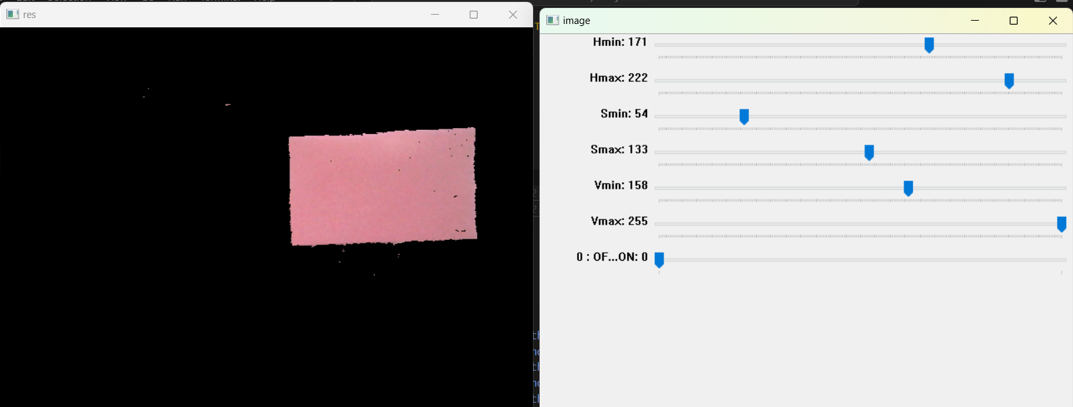
\includegraphics[width=0.8\textwidth]{./images/Chapter2/FindColorBoundry}	
	\caption[]{}
	\label{ColorCalibration}
\end{figure}
\noindent
\unskip

همچنین با استفاده از روشی تحت عنوان
\lr{Morphological Transformations}
که از مفهوم کرنل بهره می‌گیرد، می‌توان نویز‌های موجود در تصویر را از بین برد.

\begin{figure}[h]
	\centering
	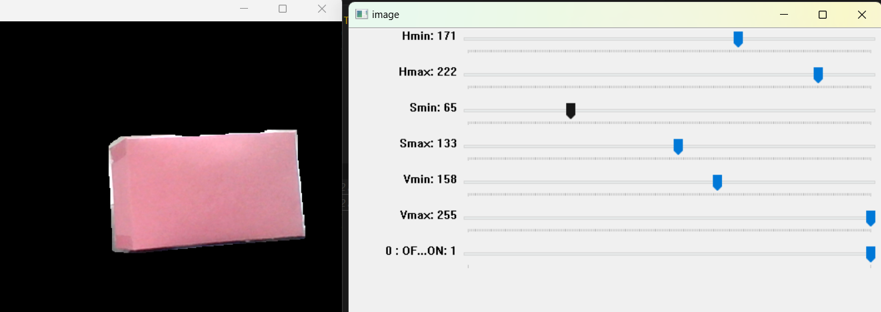
\includegraphics[width=0.8\textwidth]{./images/Chapter2/FindColorBoundryMorphologyOn}	
	\caption[]{}
	\label{ColorCalibrationMorph}
\end{figure}
\noindent
\unskip
تصویر
\ref{ColorCalibrationMorph}
حاصل استفاده از این روش بر روی تصویر
\ref{ColorCalibration}
می‌باشد.
برای این ویژگی نیز یک نوار در انتها قرار داده شده که با دستور روشن و خاموش می‌توان آن را فعال و غیرفعال کرد.
از این محدوده‌های رنگی به عنوان پارامترهای ورودی در برنامه اصلی استفاده خواهد شد که جزئیات آن در قسمت‌های آتی بیان می‌گردد.
در نتیجه اطلاعات تشخیص موانع از این مرحله استخراج شده و ربات می‌تواند بر اساس آن‌ها تصمیمات خود را در مورد حرکت و انجام وظایف مختلف بگیرد.


\subsection{تشخیص لبه‌ها}

در مرحلة تشخیص لبه‌ها، از تکنیک‌های پردازش تصویر برای تعیین مرزها و لبه‌های اشیا (موانع) استفاده می‌شود. این مرحله به‌وسیلة کانتورها آغاز می‌شود که در مرحلة قبلی به دست آمده‌اند. با استفاده از کانتورها، می‌توان مرزهای شیء را تشخیص داد و اطلاعاتی مانند عرض و ارتفاع شیء (موانع) را به دست آورد. این اطلاعات می‌توانند برای موارد مختلف مورداستفاده قرار گیرند.
به‌عنوان‌مثال می‌توانند یک معیار برای تعیین فاصله از شیء موردنظر استفاده شوند.
در نهایت با استفاده از بازه‌های تعیین شده برای رنگ‌ موانع و لبه‌ها قادر به تشخیص موانعی از آن دست در محیط باشیم.

نتیجه تشخیص موانع در فصل آخر بررسی شده است. شکل
\ref{PinkDetected}
نمونه‌ای از تشخیص مانعی به رنگ صورتی است. 

% \subsubsection{تشخیص کانتور‌ها به کمک تشخیص}
\subsection{شبه‌کد و تشریح جزئیات آن}
در زیر شبه‌کد این بخش مختصرا قرار داده شده و پس از آن به تشریح کامل‌تر آن پرداخته خواهد شد.
\section*{}
\begin{latin}
	\lstinputlisting[style=python_style]{code/Pseudocodes/ColorDetectionPseudocode.py}
\end{latin}

\section{الگوریتم درخت جستجوی تصادفی}
در بخش
\ref{مروری بر الگوریتم‌های مسیریابی}
مروری بر الگوریتم‌های مسیریابی انجام گرفت و به اهمیت این موضوع در رباتیک اشاره گردید.
پیشرفت‌های قابل توجه در الگوریتم‌های برنامه‌ریزی مسیر به ربات‌های خودکار امکان می‌دهد تا به طور کارآمد در محیط‌های پیچیده حرکت کنند. از میان این الگوریتم‌ها، الگوریتم 
\textbf{درخت جستجوی تصادفی}
\noindent\unskip\LTRfootnote{Rapidly Exploring Random Tree}
یا به اختصار
\lr{RRT}
به‌عنوان یک رویکرد نوآورانه شناخته می‌شود که به حل چالش یافتن مسیرهای قابل‌اجرا در فضاهای تنظیم با بعد بالا می‌پردازد.

این الگوریتم با استفاده از جستجوی تصادفی فضای پیکربندی به حل برنامه مساله‌ریزی مسیر می‌پردازد. در این روش، ریشه درخت در پیکربندی اولیه قرار دارد. ابتدا یک نقطه به‌صورت تصادفی با توزیع یکنواخت
\noindent\unskip\LTRfootnote{Uniform distribution}
انتخاب می‌شود. اگر نقطه انتخاب شده به فضای موانع تعلق داشته باشد، نقطه دیگری انتخاب می‌شود. با انتخاب نقطه از فضای آزاد، در راستای خط واصل بین این نقطه و ریشه درخت، نقطه جدیدی تحت عنوان
\lr{X\_new}
که به‌اندازه گام ربات از ریشه فاصله دارد، انتخاب می‌شود.
اگر بتوان
\lr{X\_new}
را با پاره‌خطی که تماماً به فضای آزاد تعلق دارد، به ریشه وصل کرد،
\lr{X\_new}
به عنوان گره جدید به درخت اضافه می‌شود.
\newpage
نمایی از درخت توسعه‌یافته با این روش در شکل
\ref{RRT}
نمایش‌داده‌شده است.
\begin{figure}[h]
	\centering
	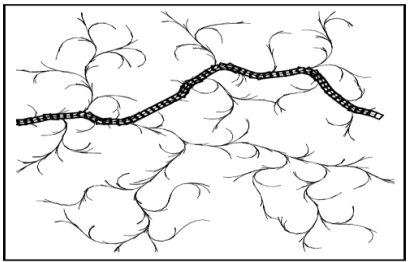
\includegraphics[width=0.6\textwidth]{./images/Chapter2/RRT}	
	\caption[الگوریتم \lr{RRT}]{الگوریتم \lr{RRT} \cite{irscholar20727638}}
	\label{RRT}
\end{figure}
\noindent
\unskip
%این الگوریتم به عنوان یک روش مبتنی بر هیوریستیک
% \noindent\unskip\LTRfootnote{Heuristic}
%، با استفاده از تصادف و کاوش به سرعت یک ساختار مانند درخت را ایجاد می‌کند که این امر آن را برای کاربردهای بهینه‌سازی زمان و محیط‌های پویا مناسب می‌کند. اصول اساسی این الگوریتم در قابلیت اکتشاف مؤثر فضاهای تنظیمی و تنوع آن، آن را به یک اصول اصلی در تحقیقات و کاربردهای رباتیک مدرن تبدیل کرده است.

%الگوریتم
%\lr{RRT}
%که در حوزه‌ی برنامه‌ریزی حرکت معرفی شده است، یک راه حل نوین برای چالش پیچیده یافتن مسیر برای عوامل خودکار در فضاهای با بعد بالا ارائه می‌دهد. در اصل، این روش به دنبال برقراری تعادل بین کاوش و بهره‌برداری می‌گردد. این الگوریتم با یک تنظیم اولیه آغاز می‌شود و به صورت تکراری با نمونه‌برداری تصادفی از نقاط در فضای تنظیمی، آن‌ها را به نزدیک‌ترین نقطه در درخت موجود متصل می‌کند. این رویکرد تضمین می‌کند که الگوریتم مناطقی از فضا را که هنوز کاوش نشده‌اند، کاوش کند، در عین حال به طور تدریجی از مناطقی که قبلاً کاوش شده‌اند بهره‌برداری می‌کند.

%یکی از ویژگی‌های برجسته‌ی
%\lr{RRT}
%توانایی تطبیق به محیط‌ها و محدودیت‌های مختلف است. با تشکیل تک تک نقاط درخت به طور تدریجی، رشد الگوریتم به سمت مناطقی با کاوش کمتر سوق می‌شود، که این ویژگی آن را به ویژه برای موقعیت‌هایی که فضای تنظیم مشخص نشده یا با موانع پراکنده است، مناسب می‌کند. علاوه بر این،
%\lr{RRT}
%همگام‌سازی سریع را اجرا می‌کند که به آن اجازه می‌دهد که مسیرهای قابل اجرا را به سرعت ایجاد کند، حتی در محیط‌های پیچیده و پویایی.

%قابلیت‌های این الگوریتم در کاربردهای زمان‌واقع واقعی نیز یک جنبه جذاب دیگر است. به دلیل ساختار تکراری و تطبیق‌پذیری، این الگوریتم برای مواردی که تصمیم‌گیری باید سریع و واکنش‌پذیر باشد، مناسب است. علاوه بر این، محققان اقدام به توسعه
%\lr{RRT}
%برای مواجهه با چالش‌های خاص، مانند موانع پویا و سیستم‌های چندعاملی و... کرده‌اند که بیشتر نشان می‌دهد چقدر این الگوریتم چندمنظوره و عملی است.

%به عبارتی، الگوریتم
%\lr{RRT}
%یک الگوریتم نوآورانه برای برنامه‌ریزی مسیرهای خودکار است. با ترکیب کاوش و بهره‌برداری ،
%\lr{RRT}
%به طور موثر در فضاهای تنظیمی با بعد بالا حرکت کرده و به شکل مناسبی به شرایط محیطی مختلف تطبیق می‌یابد. چندمنظورگی، قابلیت‌های زمان‌واقع و تطبیق‌پذیری با چالش‌های خاص،
%\lr{RRT}
%را به یک ابزار ارزنده در تحقیقات و کاربردهای رباتیک مدرن تبدیل کرده است و پیشرفت‌هایی در خودکاری، کارایی و ایمنی ایجاد می‌کند.


\subsection{شبیه‌سازی دوبعدی با پایتون}


\subsubsection{شبه‌کد و تشریح جزئیات برنامه}
در زیر شبه‌کد این بخش مختصرا قرار داده شده و پس از آن به تشریح کامل‌تر آن پرداخته خواهد شد.
\section*{}
\begin{latin}
	\lstinputlisting[style=python_style]{code/Pseudocodes/RRTPseudocode.py}
\end{latin}

همان‌طور که در شبه‌کد بالا مشخص است برنامه تا زمانی که آخرین گره گراف به ناحیه نزدیک نقطه هدف نرسد ادامه خواهد داشت. جزئیات و نحوه تولید مسیر در قطعه برنامه‌ای در پیوست موجود است. نحوه عملکرد توابع اصلی برنامه برای تولید مسیر به شرح زیر است:
\begin{enumerate}
	\item
	تولید یک گره تصادفی با فاصله مشخص از گره شروع
	\item
	بررسی معتبر بودن گره جدید (معتبر بودن به معنای آنکه آیا گره جدید بر روی موقعیت یکی از موانع نبوده باشد.)
	\item
	در صورت معتبر بودن گره جدید با فواصل از پیش تعیین شده توسط چند قدم یال‌هایی برای گراف ایجاد می‌شود.
	\item
	اگر در طی این چند قدم یکی از یال‌ها با یکی از موانع برخورد داشته باشد، قدم دیگری برای رسیدن به گره جدید انتخاب می‌شود. در غیر این صورت برنامه تا رسیدن به گره جدید ادامه داده و دوباره به مرحله اول(تولید گره تصادفی) برگشت داده خواهد شد.
	\item
	گراف این روند را تا زمانی که به نقطه هدف نزدیک نشود ادامه داده و در نهایت با توجه به دانستن موقعیت این نقطه، مسیر بهترین مسیر از بین مسیر‌های ساخته شده توسط گره‌های خود را انتخاب می‌کند.
\end{enumerate}

\newpage
برای درک بهتر مراحل بالا می‌توان شکل
\ref{مراحل تولید گره جدید}
را در نظر گرفت. همچنین قابل ذکر است که برای هر یک از مراحل بالا یک یا دو روش
\noindent\unskip\LTRfootnote{Method}
در ماژول نوشته شده در نظر گرفته شده است و این روش‌ها با یکدیگر در ارتباط بوده و یا به صورت تو در تو
\noindent\unskip\LTRfootnote{Nested}
در یکدیگر استفاده شده‌اند. 
\begin{figure}[H]
	\centering
	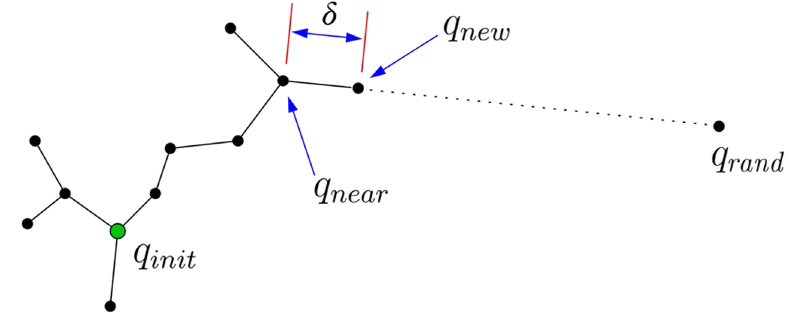
\includegraphics[width=0.8\textwidth]{./images/Chapter2/NewNodeSteps_without_background}	
	\caption[مراحل تولید گره جدید و تشکیل مسیر]{مراحل تولید گره جدید و تشکیل مسیر\cite{Algobotics}}
	\label{مراحل تولید گره جدید}
\end{figure}
\noindent
\unskip
نتایج حاصل از این شبیه‌سازی در شکل
\ref{نتیجه شبیه‌سازی RRT}
قابل مشاهده می‌باشد.
\subsubsection{ادغام الگوریتم با قابلیت‌های ربات به منظور پیاده‌سازی}
همان‌طور که مشخص است استفاده از الگوریتم پیشنهادی به تنهایی مفید واقع نخواهد شد و بایستی از قابلیت های موجود در ربات برای بهینه‌سازی این روش استفاده شود. از قابلیت های ربات که می‌تواند به کار آید، دوربین استفاده شده می‌باشد. با استفاده از دوربین موجود موانع و فاصله‌ی ربات تا موانع تشخیص داده شده و سپس با توجه به این اطلاعات ربات تصمیم می‌گیرد تا نقاط تصادفی خود را در کدام جهت تولید کند و یا در کدام جهت به تولید ادامه مسیر نپردازد. بدین منظور در بخش های آتی به تشریح موارد ذکر شده پرداخته خواهد شد.

\section{\lr{Localization}}

مکان‌یابی یکی از جنبه‌های حیاتی در علم رباتیک است که به ربات‌ها امکان می‌دهد تا مکان و موقعیت دقیق خود را در محیط تعیین کنند. برای ربات‌ها، داشتن اطلاعات صحیح و دقیق در مورد مکان خود بسیار مهم است تا بتوانند به درستی عمل کرده و وظایف مختلفی را انجام دهند. در این بخش به مکان‌یابی در ربات عنکبوتی چهارپا پرداخته خواهد‌شد. بدین منظور به انتخاب یکی از روش‌‌‌های نوین در این حوزه دست زده شد. در سال های اخیر برخی از آزمایشگاه های رباتیک در دانشگاه‌‌‌های معتبر جهان که از میان آنها می‌توان به آزمایشگاه رباتیک اپریل
\noindent\unskip\LTRfootnote{APRIL robotics lab}
در دانشگاه میشیگان اشاره کرد، روش‌هایی برای مکان‌یابی با استفاده از تگ‌هایی مشابه به تگ‌های معروف که با نام 
\textbf{کیوآر کد}
\noindent\unskip\LTRfootnote{QR code}
شناخته شده‌اند، معرفی کرده اند.

\begin{figure}[h]
	\centering
	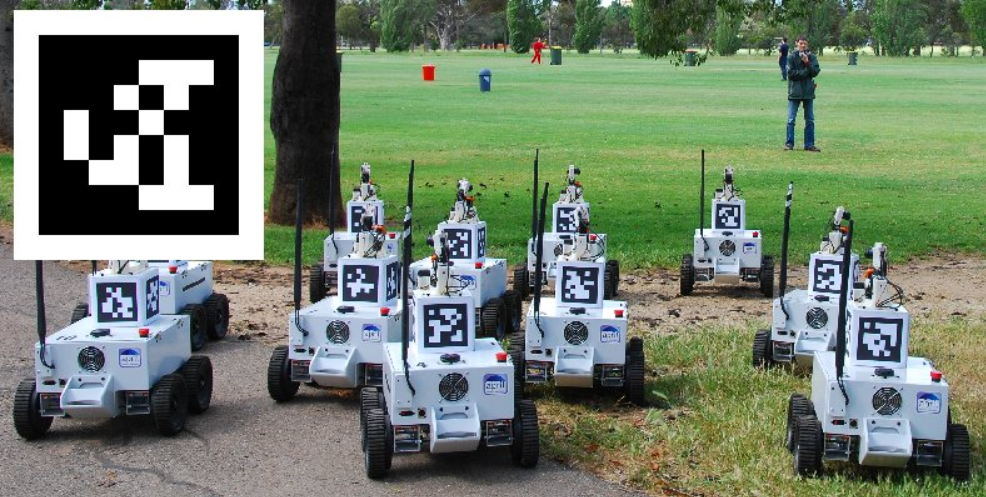
\includegraphics[width=0.8\textwidth]{./images/Chapter2/AprilTagLab}	
	\caption[آزمایشگاه اپریل میشیگان]{ آزمایشگاه اپریل میشیگان\cite{Apriltag}}
	\label{AprilTagLab}
\end{figure}
\noindent
\unskip

\subsection{استفاده از تگ}
\subsubsection{مفاهیم اصلی}
نحوه استفاده از تگ‌های این چنینی بر اساس روابط مثلثاتی و هندسه اقلیدسی موجود در فضا است و با داشتن اطلاعاتی همچون فاصله کانونی دوربین و مرکز آن، اطلاعاتی همچون فاصله در هر سه محور و یا زاویه دوربین نسبت به تگ را برمی‌گردانند.
بدین منظور از یکی از ماژول‌های موجود در کتابخانه‌ی
\lr{OpenCV}
که
\lr{Aruco}
نام دارد، استفاده خواهد شد. 
\subsubsection{شبه‌کد و تشریح جزئیات برنامه}

در زیر شبه‌کد این بخش مختصراً قرار داده شده و پس از آن به تشریح کامل‌تر آن پرداخته خواهد شد.
\section*{}
\begin{latin}
	\lstinputlisting[style=python_style]{code/Pseudocodes/ArucoPseudocode.py}
\end{latin}

مکان‌یابی در رباتیک به وسیله مختصات مکانی (مثلاً نقاط
\lr{(x, y, z)}
یا مختصات خروجی (طول، عرض، ارتفاع) صورت می‌پذیرد. این اطلاعات توسط تگ‌های
\lr{Aruco}
به ربات ارائه می‌شود. این تگ‌ها اطلاعاتی را شامل می‌شوند برای مثال سه زاویه
\lr{(roll, pitch, yaw)}
برای جهت‌یابی و فاصله‌ها در سه محور مختلف می‌شوند. برای دقت بیشتر در محاسبات، ما یک ماتریس را تعریف می‌کنیم که حاوی فاصله‌های مرکزی دوربین و فوکوس آن است و این ماتریس را به کد مکان‌یابی ارائه می‌دهیم. این اطلاعات به ربات امکان می‌دهند تا موقعیت و جهت خود را با دقت بیشتری تعیین کنند و وظایف خود را انجام دهند.
\section*{}
\begin{latin}
	\lstinputlisting[style=python_style]{code/Localization/Aruco.py}
\end{latin}

باتوجه‌به شبه‌کد و توضیحات ارائه شده، نتایج مطلوب برای مکان‌یابی ربات به‌دست‌آمد. جزئیات بیشتر آن در بخش
\ref{نتایج مکان‌یابی}
قابل‌مشاهده است.

\section{جمع بندی}
در این فصل با تشریح مفاهیمی از تصویر و پردازش آن و کاربرد‌های آن در زمینه‌های مختلف همچون رباتیک آغاز و با بررسی الگوریتم درخت جستجوی تصادفی و شبیه‌سازی آن در محیط پایتون ادامه یافت. همچنین در انتها به بررسی مفهومی بسیار مهم به نام مکان‌یابی که برای پیاده‌سازی عملی الگوریتم بر روی ربات در محیط آزمایشگاهی ضروری است اشاره و از راهکاری نوین که در سال‌های اخیر مورد‌توجه قرار گرفته است، استفاده شد.
